\documentclass[11pt]{scrartcl}

% ---------- Packages ----------
\usepackage[margin=1in]{geometry}
\usepackage{mathpazo}
\usepackage{amsmath,amssymb,amsthm}
\usepackage{tikz}
\usetikzlibrary{arrows.meta,positioning}
\usepackage[most]{tcolorbox}
\usepackage{xcolor}
\usepackage{hyperref}

% ---------- Colors ----------
\definecolor{accentblue}{RGB}{44,95,138}
\definecolor{boxfill}{RGB}{240,245,250}
\definecolor{boxborder}{RGB}{180,200,220}
\definecolor{highlightred}{RGB}{200,50,50}

% ---------- Theorem environments ----------
\newtcolorbox{thmbox}[1]{
  colback=boxfill, colframe=boxborder,
  boxrule=0.6pt, arc=2pt, left=6pt, right=6pt, top=4pt, bottom=4pt,
  fonttitle=\bfseries\color{accentblue}, title=#1
}
\theoremstyle{plain}
\newtheorem{theorem}{Theorem}
\theoremstyle{remark}
\newtheorem*{remark}{Remark}

\hypersetup{colorlinks=true, linkcolor=accentblue, urlcolor=accentblue}

\title{\color{accentblue}Connectivity in Graphs}
\author{}
\date{}

\begin{document}
\maketitle

% =========================================================
\begin{thmbox}{Theorem 1}
A graph $G$ is bipartite $\iff$ every cycle of $G$ has even length.
\end{thmbox}

\begin{proof}
($\Rightarrow$) Since $G$ is bipartite, we can split its vertex set into two disjoint sets $A$ and $B$ so that each edge of $G$ joins a vertex of $A$ and a vertex of $B$. Let $v_0 \to v_1 \to \cdots \to v_n \to v_0$ be a cycle of $G$, and assume $v_0 \in A$; then $v_1 \in B$, $v_2 \in A$, and so on. Since $v_n$ must lie in $B$, the cycle has even length.

\medskip
\noindent ($\Leftarrow$) Pick any vertex $u \in V(G)$, and define two sets
$$X = \{x \in V : d(u,x) \text{ is even}\}, \qquad Y = \{y \in V : d(u,y) \text{ is odd}\},$$
where $d(u,x)$ denotes the length of a shortest path from $u$ to $x$. We claim $(X,Y)$ is a bipartition, i.e.\ no edge connects two vertices of $X$ or two vertices of $Y$.

Suppose, for contradiction, that there exists an edge connecting two vertices in the same set, say $v, w \in X$. Let $P$ be a shortest path from $u$ to $v$, and $Q$ a shortest path from $u$ to $w$. Denote by $u_L$ the last common vertex of $P$ and $Q$ (where the two paths diverge), so that
$$P = u \to \cdots \to u_L \to P_1 \to v, \qquad Q = u \to \cdots \to u_L \to Q_1 \to w.$$
Both $P$ and $Q$ have the same length up to $u_L$; since the lengths of $P$ and $Q$ are both even, the lengths of $P_1$ and $Q_1$ are also even (because each total is even). Now consider the path $P_1 + \overline{Q_1} + (v,w)$ (i.e.\ $P_1$, followed by $Q_1$ reversed, followed by the edge $(v,w)$): this is a cycle of odd length, a contradiction.

The same argument applies to the set $Y$.

\begin{center}
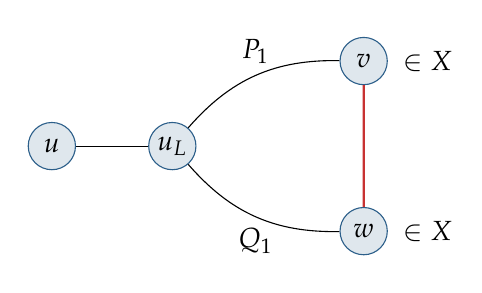
\begin{tikzpicture}[scale=0.9, every node/.style={circle,draw=accentblue,fill=accentblue!15,minimum size=6mm,inner sep=0pt}]
  \node (u)  at (0,0)     {$u$};
  \node (ul) at (1.7,0)   {$u_L$};
  \node (v)  at (4.4,1.2) {$v$};
  \node (w)  at (4.4,-1.2){$w$};

  \draw (u)--(ul);
  \draw (ul) to[bend left=25]  node[above,midway,draw=none,fill=none]{$P_1$} (v);
  \draw (ul) to[bend right=25] node[below,midway,draw=none,fill=none]{$Q_1$} (w);
  \draw[highlightred, thick] (v)--(w);

  \node[draw=none,fill=none] at (5.3,1.2)  {$\in X$};
  \node[draw=none,fill=none] at (5.3,-1.2) {$\in X$};
\end{tikzpicture}
\end{center}
\end{proof}

% =========================================================
\begin{thmbox}{Theorem 2}
Let $G$ be a simple graph on $n$ vertices. If $G$ has $k$ components, then the number $m$ of edges of $G$ satisfies
$$n - k \leq m \leq \frac{(n-k)(n-k+1)}{2}.$$
\end{thmbox}

\begin{proof}
We prove the lower bound $m \geq n-k$ by induction on the number of edges; the result is trivial if $G$ is a null graph. If $G$ contains as few edges as possible (say $m_0$) subject to having $n$ vertices and $k$ components, then the removal of any edge of $G$ must increase the number of components by $1$, and the remaining graph has $n$ vertices, $k+1$ components, and $m_0 - 1$ edges. By the induction hypothesis,
$$m_0 - 1 \geq n - (k+1) \implies m_0 \geq n-k,$$
as required.

\medskip
\noindent To prove the upper bound, we assume that each component of $G$ is complete. Suppose there are two components $C_i, C_j$ with $n_i$ and $n_j$ vertices respectively, $n_i \geq n_j \geq 1$. If we replace $C_i$ and $C_j$ by complete graphs on $n_i+1$ and $n_j-1$ vertices, then the total number of edges
$$\frac{(n_i+1)(n_i)}{2} + \frac{(n_j-1)(n_j-2)}{2}$$
is increased by $n_i - n_j + 1 > 0$. It follows that, in order to maximize the number of edges, $G$ must consist of a complete graph on $n-k+1$ vertices together with $k-1$ isolated vertices, which gives
$$\frac{(n-k+1)(n-k)}{2} + 0 \times (k-1).$$
\end{proof}

% =========================================================
\begin{thmbox}{Corollary 3}
Any simple graph with $n$ vertices and more than $\dfrac{(n-1)(n-2)}{2}$ edges is connected.
\end{thmbox}

\begin{proof}
By Theorem 2,
$$\frac{(n-1)(n-2)}{2} \geq \frac{(n-k)(n-k+1)}{2}, \qquad \forall\, k \geq 2,$$
which implies $k = 1$.
\end{proof}

\end{document}
